\documentclass{article}
\usepackage[utf8]{inputenc}
\usepackage{listings}
\usepackage{graphicx}
\usepackage{color}
\usepackage{placeins}

\title{Where Favorite Characters go to Die}
\author{Erin Pierce and Ben Kahle}
\date{October 2014}

\begin{document}

\maketitle

\section{Predicting Deaths}
The \textit{A Song of Ice and Fire} series by George R. R. Martin is notorious for its high frequency of character deaths. Using data from the first five books of the series we create a model of death probabilities that allow us a rough extrapolation into the potential death probabilities of the final two books. Given the conclusive nature of the final books, it is reasonable to assume that a trend determined from the currently released material will not hold true, however this problem still provides an interesting opportunity to explore survival curves in fictional worlds. Additionally, our model opens the possibility of exploring the survival probability of a hypothetical character in the first five books, given specific characteristics such as royal loyalties and character gender.

\section{Data Source}
The data we create the model with is from the website "A Wiki of Ice and Fire" (http://awoiaf.westeros.org/index.php/List\_of\_characters). This wiki contains fairly detailed accounts of the roles of even minor characters from the series. By scraping this site we find that out of 971 recorded characters, 295 characters die at some point in the first five books. We determine the "age" of characters as the number of books from their introduction to either their death, or through the fifth book.

\section{Building a Bayesian Model}
We are using a Weibull distribution to model a survival curve for characters in the series.  Weibull distributions have two parameters, k and lambda, which control the shape of the curve.  The inverse of the CDF of the Weibull distribution is the survival curve.  This survival curve, evaluated at a certain character's age, is the probably that a character will have a lifetime greater than that age.  The PDF of the Weibull distribution, evaluated at a certain character's age, is the probability that a character had a lifetime that long. We start with a uniform prior, where k is equally likely to fall between 0.1 and 6, and lambda is equally likely to fall between 0.1 and 6.  For each character in our data set, we calculate how 'old' they are (or were, at their time of death).  Currently, these ages have a resolution in books. For each k and lambda, we then seek to determine how good that Weibull is at predicting the characters life or death. For alive characters we calculate the CDF at their age, and for dead characters we evaluate the PDF at their age.  For every character, we then have a probability associated with each value of k and lambda, essentially how well that specific Weibull predicts their status.  We then use this probability to update our beliefs.  After doing this for every character, we get a marginal distribution for k and lambda.

We use the following Python class to encapsulate the above procedure for updating the belief of each pair of k and lambda values successfully predicting the death of each character:



\lstset{language=Python,
        numbers=left,
        frame=single,
        morecomment=[l]{//},
        backgroundcolor=\color{white},   % choose the background color t
        basicstyle=\footnotesize,        % size of fonts used for the code
        breaklines=true,                 % automatic line breaking only at whitespace
        captionpos=b,                    % sets the caption-position to bottom
        commentstyle=\color{mygreen},    % comment style
        escapeinside={\%*}{*)},          % if you want to add LaTeX within your code
        keywordstyle=\color{blue},       % keyword style
        stringstyle=\color{mymauve},     % string literal style
        basicstyle=\footnotesize\ttfamily % fixed-width font
}
\begin{lstlisting}
class GOT(thinkbayes2.Suite, thinkbayes2.Joint):

  def Likelihood(self, data, hypo):
    age, alive = data
    k, lam = hypo
    if alive:
      prob = 1-exponweib.cdf(age, k, lam)
    else:
      prob = exponweib.pdf(age, k, lam)
    return prob

def Update(k, lam, age, alive):
  joint = thinkbayes2.MakeJoint(k, lam)
  suite = GOT(joint)
  suite.Update((age, alive))
  k, lam = suite.Marginal(0, label=k.label), suite.Marginal(1, label=lam.label)
  return k, lam
\end{lstlisting}



\lstset{language=Python,
        numbers=left,
        frame=single,
        morecomment=[l]{//},
        backgroundcolor=\color{white},   % choose the background color t
        basicstyle=\footnotesize,        % size of fonts used for the code
        breaklines=true,                 % automatic line breaking only at whitespace
        captionpos=b,                    % sets the caption-position to bottom
        commentstyle=\color{mygreen},    % comment style
        escapeinside={\%*}{*)},          % if you want to add LaTeX within your code
        keywordstyle=\color{blue},       % keyword style
        stringstyle=\color{mymauve},     % string literal style
        basicstyle=\footnotesize\ttfamily % fixed-width font
}

\begin{figure}[ht!]
\centering
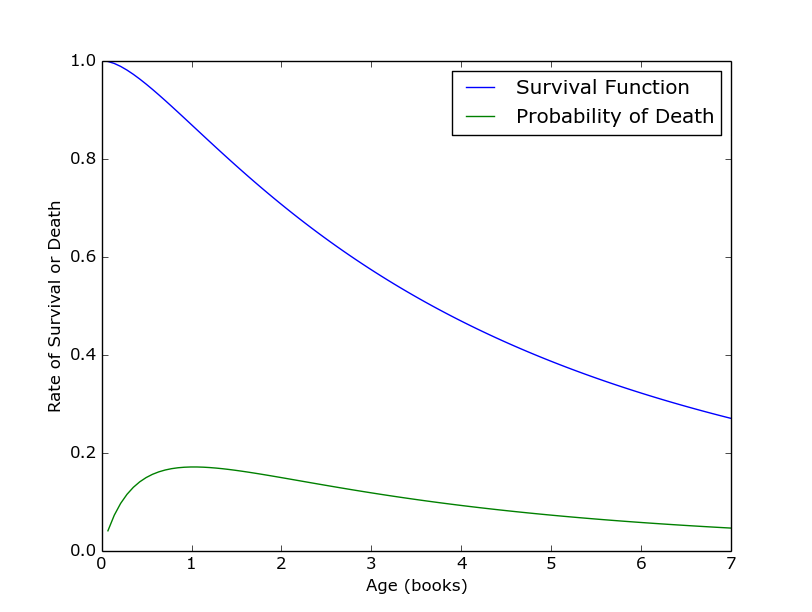
\includegraphics[width=\textwidth]{weibulldistr.png}
\caption{The survival function (blue) and rate of death (green) from the Weibull Distribution calculated using the mean of the k and lambda distributions after updates.}
\end{figure}

\newpage

\section{Analyzing the Model}

To check the results of the updated data, we find the mean of the marginal distributions of k and lambda and plot the survival function and the PDF of the inverse of the survival function given that set of k and lambda as can be seen in Figure 1. Two promising aspects of the survival function are the number number of characters alive after zero books, 100\%, and the fact that there are a decent number of characters alive at the end of the seven book range. These results demonstrate that all characters live for at non-zero length of time and that not all characters die by the end of the series, as is expected (despite some reader's insistence of the contrary). Additionally, we can see that the majority of characters die after only one book, while characters who live longer have a lower chance of death. This results from many lesser characters being introduced only shortly before their death in large battles or other scenes where many characters are killed. More important characters who survive further into the series however, tend to have larger roles to play and thus have a lower rate of death. The extrapolation into books six and seven in this plot are unfortunately ignorant to major plot chances which may result in the deaths of many major characters which would cause a discontinuous drop in the survival function.

\begin{figure}[ht!]
\centering
\includegraphics[width=\textwidth]{K_lam_dist.png}
\caption{This shows our PDFs for k and lambda after updating with all the characters.  The x-axis is values for k and lambda and the y-axis is the probability.}
\end{figure}

\section{Validating the Model with Kaplan-Meyer Estimation}
Using classical statistics, we take our data set and perform a Kaplan-Meyers estimation. Kaplan-Meyers is way of looking at how many people are at risk of death in a population for each time step versus how many actually die at that juncture. This sort of estimation does good job of portraying what happened in the first five books, but does not lend itself well to extrapolation into future novels. This estimation yields the hazard curve and survival function seen in Figures 3 and 4. While the Weibull distribution we calculated through Bayesian updates and the survival function calculated by the Kaplan-Meyes estimation are not perfect matches, the similar shape and overall curve suggests that they both provide a reasonable model of the life and death data. The Kaplan-Meyers hazard function demonstrates a similar reduction in death rates to what is seen in the Weibull distribution survival function. The similarity between the two models offers validation that the Weibull Distribution parameters chosen provide a reasonable estimation of the character data and as such can be reasonable used to extrapolate to the sixth and seventh books of the series. 

\begin{figure}[ht!]
\centering
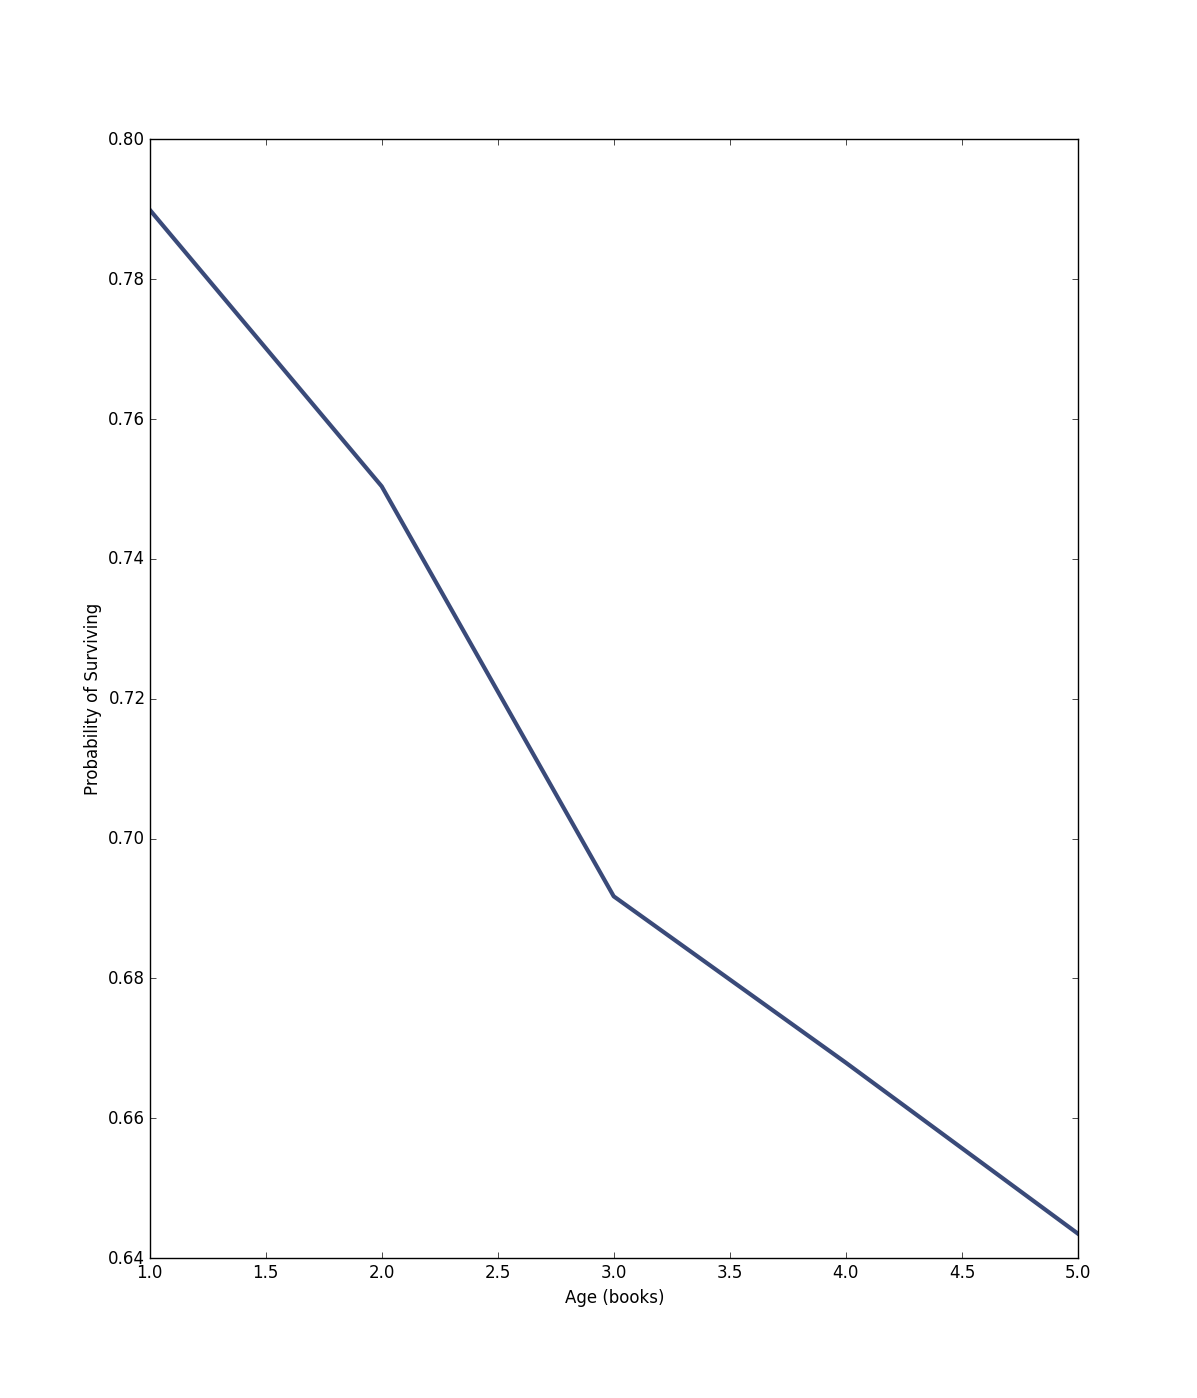
\includegraphics[width=\textwidth]{survivalfunction.png}
\caption{The survival function as calculated using a Kaplan-Meyers estimation.}
\end{figure}
\begin{figure}[ht!]
\centering
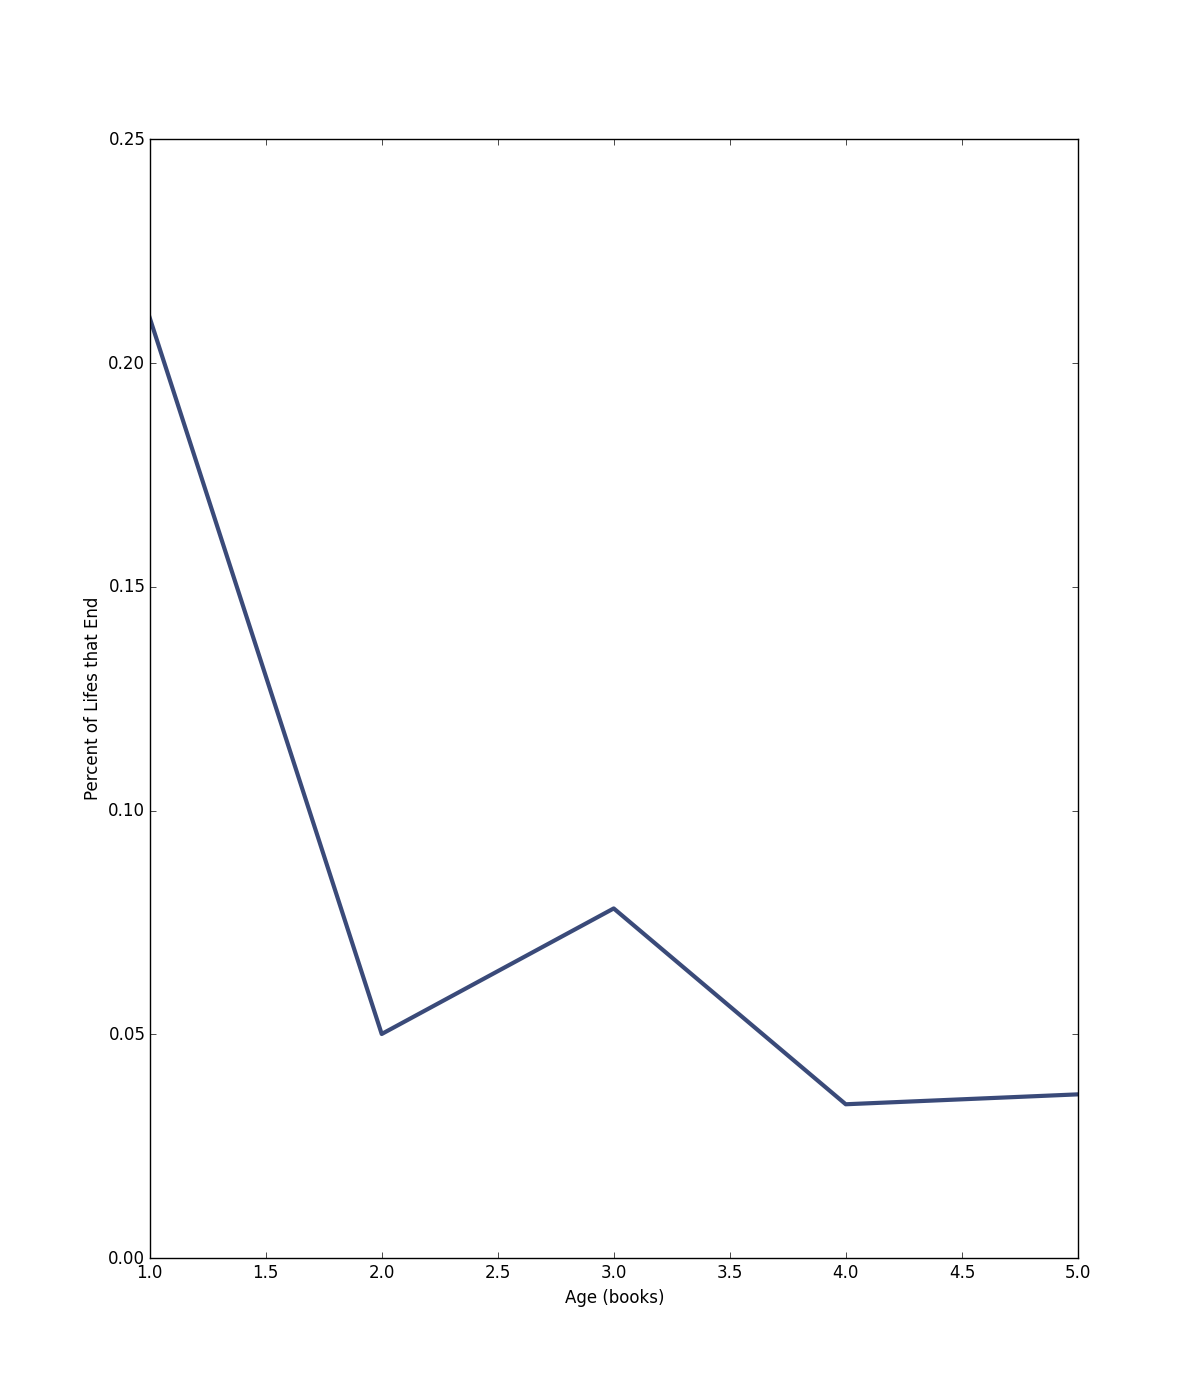
\includegraphics[width=\textwidth]{hazardfunction.png}
\caption{The hazard function as calculated using a Kaplan-Meyers estimation.}
\end{figure}

\newpage

\section{Extensions of this Study}
There are a number of steps to take improve the accuracy of our model as well as derive more value from the predictions. The first order of business is to flush out the data set so that we know the exact chapter of every characters introduction, and in some cases, the chapter of their death. We have started to gather this data, but are not done yet. This greater resolution on our data should lead to some interesting results, and help reduce the granularity of our predictions. At this point we would also like to create separate survival curves for different combinations of houses loyalties, genders, and social status. These separate survival curves will allow us to create more specific predictions rather than looking at all characters in the series at once. Once this is finished, we intend to augment and further revise this report, such that it might be suitable for a blog post.That time is not now.

The code used in the case study can be found at: \\
http://github.com/benkahle/bayesianGameofThrones

\section{Puppy of the Week}
\begin{figure}[ht!]
\centering
\includegraphics[width=.75\textwidth]{shame_of_cones.jpg}
\caption{The Bayesian Game of Thrones mascot}
\end{figure}

\end{document}